	\documentclass[10pt,oneside]{CBFT_book}
	% Algunos paquetes
	\usepackage{amssymb}
	\usepackage{amsmath}
	\usepackage{graphicx}
	\usepackage{libertine}
% 	\usepackage[bold-style=TeX]{unicode-math}
	\usepackage{lipsum}

	\usepackage{natbib}
	\setcitestyle{square}

	\usepackage{polyglossia}
	\setdefaultlanguage{spanish}
	



	\usepackage{CBFT.estilo} % Cargo la hoja de estilo

	% Tipografías
	% \setromanfont[Mapping=tex-text]{Linux Libertine O}
	% \setsansfont[Mapping=tex-text]{DejaVu Sans}
	% \setmonofont[Mapping=tex-text]{DejaVu Sans Mono}

	%===================================================================
	%	DOCUMENTO PROPIAMENTE DICHO
	%===================================================================

\begin{document}

% =================================================================================================
\chapter{Conceptos fundamentales de electromagnetismo}
% =================================================================================================


% =================================================================================================
% \section{Ecuaciones de Maxwell}
% =================================================================================================

La idea del curso es resolver las ecuaciones que describen matemáticamente el comportamiento clásico 
de los campos electromagnéticos, es decir las ecuaciones de Maxwell, en diversas situaciones.
Luego, la conexión con la fuerza que experimentarán las partículas cargadas por la acción de dichos
campos vendrá descripta por la fuerza de Lorentz.

Panorámicamente, lo dicho corresponde a trabajar con el set de ecuaciones
\[
	\divem{D} = 4 \pi \rho_\ell \qquad \divem{B} = 0 
\]
\[
	\rotorm{E} = - \frac{1}{c} \dpar{\vb{B}}{t} 
	\qquad 
	\rotorm{H} = \frac{4\pi}{c} \vb{J}_\ell + \frac{1}{c}\dpar{\vb{D}}{t},
\]
las cuales permiten determinar a los campos $\vb{E}, \vb{D}, \vb{B}, \vb{H}$ a partir de la densidad 
de carga $\rho$ y de corriente $\vb{J}$ (notemos que también los campos $\vb{D}$ y $\vb{B}$ influyen
en el comportamiento de $\vb{H}$ y $\vb{E}$).
Finalmente, la fuerza de Lorentz que actúa sobre una partícula de carga $q$ que se mueve con velocidad
$\vb{v}$ es
\[
	\vb{F} = q \left( \vb{E} + \frac{1}{c} \pv{v}{B} \right).
\]

Crudamente podemos decir que de esto trata el electromagnetismo clásico.
Las ecuaciones de Maxwell son lineales, de modo que vale la superposición aunque los campos tienen en
sí matemáticamente naturaleza diferente.
Los campo $\vb{E}, \vb{D}$ don ejemplos de vectores polares (aquellos que tienen bien definido el sentido,
como la fuerza, la posición y la velocidad) mientras que $\vb{B}, \vb{H}$ son ejemplos de vectores axiales,
que por el contrario tienen su sentido definido por una convención, como por ejemplo las velocidades
angulares.

\notamargen{Siempre usamos terna derecha.}

De acuerdo con ello, el carácter de vector axial o polar tiene consecuencias en la transformación de
los mismos. Las transformaciones que se considerarán serán rotaciones, reflexiones espaciales y reflexiones
temporales. Las ecuaciones de Maxwell permanecen invariantes ante estas transformaciones.

\notamargen{Si multiplico vectorialmente dos vectores polares obtengo un vector axial.}

% Son ecuaciones lineales de modo que vale la superposición (con \vb{E}, \vb{B} y 
% cualquier vector relacionado linealmente con ellos).

El resto del capítulo recorrerá lo que es la construcción usual del electromagnetismo; primeramente considerar 
situaciones estáticas, independientes del tiempo, lo cual hace que aparezcan como fenómenos independientes la 
electricidad y el magnetismo y luego repasar someramente algunas propiedades matemáticas útiles para el
formalismo.

% =================================================================================================
\section{Electrostática}
% =================================================================================================

La ley de Coulomb establece que 
\[
	\vb{F}_{12} = k \: q_1 q_2 \frac{(\vb{x}_1 - \vb{x}_2)}{|\vb{x}_1 - \vb{x}_2 |^3}
\]
es la fuerza sobre la partícula en $\vb{x}_1$ debido a la partícula en $\vb{x}_1$. La constante $k$ está para ajustar
las unidades. En sistema gaussiano es $k=1$ y adimensional.
La Figura \ref{fig_ft1_ejescargas} ilustra la situación para el caso en que ambas cargas tienen igual signo; en ese
caso la fuerza $\vb{F}_{12}$ tiene la dirección del vector $\vb{x}_1 - \vb{x}_2$: apunta desde la fuente hacia el punto 
donde se evalúa.

\begin{figure}[!h]
	\begin{center}
	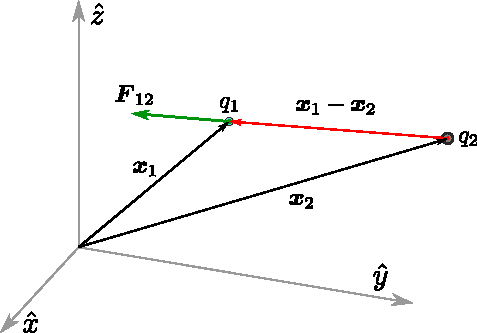
\includegraphics[width=0.5\textwidth]{images/fig_ft1_ejescargas.pdf}	 
	\end{center}
	\caption{Fuerza sobre la carga $q_1$ debida a la carga $q_2$.}
	\label{fig_ft1_ejescargas}
\end{figure} 

Cuando la carga $q_1$ es suficientemente pequeña como para no perturbar a la carga $q_2$ que origina la fuerza, se puede 
utilizar la ley de Coulomb para definir el campo eléctrico según
\[
	\vb{E}_{12}(\vb{x}_1) \equiv \lim_{q_1 \to 0} \frac{\vb{F}_{12}}{q_1}.
\]

Para una distribución discreta de $N$ cargas $q_i$ y tomando $\vb{x}_1 \equiv \vb{x}$ se tiene
\[
	\vb{E}(\vb{x}) = \sum_{i=1}^N \; q_i \frac{(\vb{x} - \vb{x}_i)}{|\vb{x} - \vb{x}_i |^3}.
\]
En el límite en que las cargas están lo suficientemente próximas como para considerar que forman se tiene una distribución
de carga de volumen $\rho(\vb{x})$, la expresión del campo adopta la forma de una integral
\[
	\vb{E}(\vb{x}) = \int_{V'} \rho(\vb{x}') \frac{(\vb{x} - \vb{x}')}{|\vb{x} - \vb{x}' |^3} \: dV' 
\]
donde $V'$ es el volumen de integración. En general \vb{x} es el llamdo punto campo y $\vb{x}'$ punto fuente.

\subsection{Conservación de la carga}

Aceptaremos el principio de conservación de la carga; la carga eléctrica no se genera ni se destruye. 
Considerando una región $\Omega$ en el espacio (cuya frontera está fija) la carga total encerrada en la
misma es 
\[
	Q(t) = \int_\Omega \rho(\vb{x}',t)\: d\Omega,
\]
siendo su variación temporal 
\[
	\dtot{Q(t)}{t} = \int_\Omega \dpar{\rho(\vb{x}',t)}{t} \: d\Omega,
\]
donde la derivada total se transforma en una derivada parcial debido a que el volumen es fijo.
\notamargen{Acá creo que la derivada debería ser la parcial desde el vamos. Check!}

La conservación de la carga nos dice que como la carga no aparece ni desaparece mágicamente, entonces
la variación de la carga contenida en $\Omega$ en cualquier instante de tiempo se debe al flujo neto de 
carga de la misma; es decir a la diferencia entre la que abandona la región y aquella que entra.
Como ilustra esquemáticamente la Figura \ref{conserv_carga}, la variación de carga $\Delta Q$ en un
dado $\Delta t$ corresponde a la diferencia entre las entrantes y las salientes.

La forma que tiene ese flujo se construye a partir del análisis ilustrado en el inserto de la figura.
Allí se ve un elemento pequeño $\delta \Omega$ que linda con la frontera de la región. Este elemento
$\delta V$ es lo suficientemente pequeño como para que en su interior el campo de velocidad de
las cargas sea constante. La {\it caja} $\delta V$ tiene un volumen que se puede expresar $\ell \delta S$
(longitud de la caja por área de la base). La longitud $\ell $ se elige como
$ \ell = v_n \delta t$, donde $v_n$ es la componente de la velocidad normal a la superficie. Así elegido, 
el volumen $\delta V = v_n \delta t \delta S$ representa el volumen que pasaría a través de $\delta S$ 
en el tiempo $\delta t$. En efecto, la partícula más lejana del borde $\delta S$ que está a distancia $\ell$ 
recorrerá en $\delta t$ justamente esa distancia (la velocidad $v$ es constante para todo el elemento).
Si la velocidad estuviese orientada hacia adentro, entonces tendríamos un bloque similar de carga 
entrante, y el razonamiento es el mismo.

La cantidad de carga $\delta Q$ que atraviesa el área $\delta S$ será entonces 
\[
	\delta Q = \rho \delta V = \rho v_n \delta S \delta t = \rho \vb{v} \cdot (\hat{n} \delta S) \delta t
\]
donde se ha expandido la velocidad normal. Entonces la variación de la carga en el elemento es
\[
	\frac{\delta Q}{\delta t} = \rho \vb{v} \cdot (\hat{n} \delta S).
\]

Si el producto escalar entre la velocidad y la normal es positivo entonces esto significa que la carga
abandona la superficie mientras que el caso contrario implica carga entrando en la misma. Entonces 
debemos ajustar la expresión anterior con un signo menos. Entonces, pasando al continuo
\[
	\dpar{Q}{t} = - \int_{\partial\Omega} \: \vb{J} \cdot d\vb{S}
\]
donde $\vb{J} = \rho \vb{v}$ es el vector densidad de corriente y $d\vb{S} = \hat{n}dS$ es el diferencial
de superficie vectorial.

Entonces, juntando las dos expresiones para la carga tenemos 
\[
	\int_\Omega \dpar{\rho(\vb{x}',t)}{t} \: d\Omega = - \int_{\partial\Omega} \: \vb{J} \cdot d\vb{S},
\]
y aplicando el teorema de la divergencia en el miembro derecho
\[
	\int_\Omega \dpar{\rho(\vb{x}',t)}{t} \: d\Omega = - \int_\Omega \: \divem{J} \: d\Omega,
\]
o bien 
\[
	\int_\Omega \left[ \dpar{\rho(\vb{x}',t)}{t} + \divem{J} \right] \: d\Omega = 0,
\]
y como esto vale para cualquier volumen $\Omega$ se sigue que el corchete debe ser nulo, de modo que se tiene
\[
	\dpar{\rho}{t} + \divem{J} = 0,
\]
que es la ecuación de continuidad de la carga.

% Entonces la carga que existe en una región depende de la tasa con la cual entra a la misma y aquella con la que la abandona.
% La carga total sale de una integral 
% \[
% 	Q = \int_{V'}  \rho(\vb{x}') dV'
% \]
% como muestra la imagen
\begin{figure}[htb]
	\begin{center}
	\includegraphics[width=0.25\textwidth]{images/fig_ft1_conserv.pdf}	 
	\end{center}
	\caption{}
	\label{conserv_carga}
\end{figure} 
% y si el volumen es fijo podemos tomar la derivada con respecto al tiempo que pasa el interior como
% derivada parcial,
% \[
% 	\dtot{Q}{t} = \int_{V'} \dpar{\rho}{t} (\vb{x}') dV' = - \int_{S\equiv\partial V'} \vb{J} \cdot d\vb{S}
% \]
% y el miembro extremo derecho  se debe a que si la carga varía es a consecuencia de que se va en
% forma de flujo. 
% Aplicando el teorema de la divergencia en el miembro derecho,
% \[
% 	\int_{V'} \dpar{\rho}{t} (\vb{x}') dV' = - \int_{V'} \nabla \cdot \vb{J} \; dV'
% \]
% lo cual vale para todo volumen y entonces esto significa que
% \[
% 	\dpar{\rho}{t} + \nabla \cdot \vb{J} = 0
% \]
% que es la ecuación de continuidad de la carga. 
\notamargen{Si fuera $\nabla \cdot \vb{J}=0$ esto significa que las líneas
de \vb{J} no tienen principio ni fin.Check!}

Si es $\divem{J}=0$ no se acumula carga; las líneas de $\vb{J}$ no tienen principio ni fin.
Los problemas de corrientes estacionarias cumplen esta condición. Esta condición en la ecuación de continuidad
nos dice que la distribución de carga no varía con el tiempo.

% =================================================================================================
\section{Interacción magnética}
% =================================================================================================

Cuando se da $\nabla \cdot \vb{J}=0$ hablamos de una corriente estacionaria (no hay acumulación de carga en
ninguna parte). Las corrientes estacionarias producen efectos magnéticos dados por la ley de Biot-Savart
\[
	\vb{B}(\vb{x}) = \frac{1}{c} \int_\Gamma \frac{I d\vb{\ell}' \times (\vb{x} - \vb{x}')}{|\vb{x} - \vb{x}'|^3} 
\]
que es válida para un circuito $\Gamma$, que es una curva --lineal-- que se recorre en sentido positivo (CCW).
Si no puede despreciarse el espesor de un circuito, hay que considerar una integral de volumen y la expresión es 
\[
	\vb{B}(\vb{x}) = 
	\frac{1}{c} \int_{V'} \frac{ \vb{J}(\vb{x}') \times (\vb{x} - \vb{x}')}{|\vb{x} - \vb{x}'|^3} \: dV'.
\]
Luego, la fuerza sobre un circuito lineal $\Gamma$ es
\[
	\vb{F} = \frac{1}{c} \int_\Gamma I d \vb{\ell} \times \vb{B},
\]
mientras que para un volumen se tiene
\[
	\vb{F} = \frac{1}{c} \int_V \vb{J} \times \vb{B} \: dV.
\]
La expresión del torque es
\[
	\vb{\Tau} = \frac{1}{c} \int_V \vb{x} \times (\vb{J} \times \vb{B}) \: dV.
\]

La transformación entre estas integrales puede hacerse merced al siguiente razonamiento,
% \begin{align*}
%  	I d\vb{\ell} \times \vb{B} = \vb{J}  \cdot d\vb{S} d\vb{\ell}  \times \vb{B} =
%   	\cos(\theta) dS \vb{J} d\ell \times \vb{B} = \\
% 	\vb{J} \times \vb{B}  \cos(\theta) dS d\ell  = \vb{J} \times \vb{B}  d\vb{S} \cdot d\vb{\ell}  = 
% 	\vb{J} \times \vb{B}  dV 
% \end{align*}
\[
  	I d\vb{\ell} \times \vb{B} = \vb{J}  \cdot d\vb{S} d\vb{\ell}  \times \vb{B} =
  	\cos(\theta) dS \vb{J} d\ell \times \vb{B} = 
\]
\[
	\vb{J} \times \vb{B}  \cos(\theta) dS d\ell  = \vb{J} \times \vb{B}  d\vb{S} \cdot d\vb{\ell}  = 
	\vb{J} \times \vb{B}  dV 
\]

\subsection{Fuerza de un circuito sobre otro}

La fuerza ejercida por el campo magnético de un circuito 2 sobre otro circuito 1 puede calcularse con un poco de 
paciencia como sigue
\[
	F_{12} = \frac{1}{c} \int_{\Gamma_1} I_1 d\vb{\ell}_1 \times \left\{
	\frac{1}{c} \int_{\Gamma_2} \frac{I_2 d\vb{\ell}_2 \times (\vb{x}_1 - \vb{x}_2)}{|\vb{x}_1 - \vb{x}_2|^3} 
	\right\}
\]
\[
	F_{12} = \frac{I_1 I_2}{c^2} \int_{\Gamma_1} \int_{\Gamma_2} d\vb{\ell}_1 \times \left\{
	\frac{d\vb{\ell}_2 \times (\vb{x}_1 - \vb{x}_2)}{|\vb{x}_1 - \vb{x}_2|^3} 
	\right\},
\]
y utilizando una identidad vectorial, 
\[
	F_{12} = \frac{I_1 I_2}{c^2} \int_{\Gamma_1} \int_{\Gamma_2} d\vb{\ell}_2  \left\{
	\frac{d\vb{\ell}_1 \cdot (\vb{x}_1 - \vb{x}_2)}{|\vb{x}_1 - \vb{x}_2|^3} 
	\right\} - \int_{\Gamma_1} \int_{\Gamma_2} \frac{ (\vb{x}_1 - \vb{x}_2)}{|\vb{x}_1 - \vb{x}_2|^3} 
	\left\{ d\vb{\ell}_1 \cdot d\vb{\ell}_2 \right\}
\]
Luego, se puede reescribir el primer término notando que 
\be
	\frac{ (\vb{x}_1 - \vb{x}_2)}{|\vb{x}_1 - \vb{x}_2|^3} = 
	\nabla_{\vb{x}_2} \frac{ 1 }{|\vb{x}_1 - \vb{x}_2|} =
	- \nabla_{\vb{x}_1} \frac{ 1 }{|\vb{x}_1 - \vb{x}_2|} ,
	\label{ident_vec_posicion}
\ee
de manera que la primer integral resulta 
\[
	- \int_{\Gamma_2} d\vb{\ell}_2 \int_{\Gamma_1} d\vb{\ell}_1 \cdot \nabla_{\vb{x}_1} \frac{ 1 }{|\vb{x}_1 - \vb{x}_2|} ,
\]
la cual es nula porque se está integrando un gradiente en una curva cerrada.
% \[
% 	\int_{\Gamma_1} d\vb{\ell}_1 \cdot \nabla_{\vb{x}_1} = 0.
% \]

Entonces, se tiene 
\[
	F_{12} = - \frac{I_1 I_2}{c^2} \int_{\Gamma_1} \int_{\Gamma_2} \frac{ (\vb{x}_1 - \vb{x}_2)}{|\vb{x}_1 - \vb{x}_2|^3} 
	\left( d\vb{\ell}_1 \cdot d\vb{\ell}_2 \right)
\]
que vale lo mismo si intercambiamos $\Gamma_1$ con $\Gamma_2$ en la integración, lo cual implica
que la fuerza sobre un circuito debida a otro es igual a la fuerza sobre este último debida al primero.
Esto quiere decir que vale el principio de acción y reacción en el caso de corrientes estacionarias.
Si las corrientes no son estacionarias no se tendrá, en general, este resultado. Con corrientes no
estacionarias se generará campo electromagnético y habrá emisión de radiación.


% =================================================================================================
\section{Teorema de Helmholtz}
% =================================================================================================

Nos dice que un campo vectorial está completamente determinado por su divergencia y su rotor.
Por ejemplo, para un campo eléctrico se tiene 
\[
	\vb{E} = \int_{V'} \rho \frac{\vb{x} - \vb{x}'}{|\vb{x} - \vb{x}'|^3} dV' = 
		- \int_{V'} \rho \nabla_{\vb{x}} \frac{ 1 }{|\vb{x} - \vb{x}'|} dV' = 
		- \nabla_{\vb{x}} \int_{V'}   \frac{ \rho }{|\vb{x} - \vb{x}'|} dV' = 
\]
donde la integral que ha resultado dentro del gradiente es la integral de Poisson. Entonces,
\[
	\vb{E} = - \nabla_{\vb{x}} \phi (\vb{x}),
\]
de modo que $\vb{E}$ es un gradiente y por ello 
\[
	\nabla  \times \vb{E} = 0.
\]

Esta última condición implica que el campo electrostático $\vb{E}$ es conservativo, cumple 
$\oint_\Gamma \vb{E}\cdot d\vb{\ell} = 0$, o lo que es lo mismo, $\vb{E}$ es irrotacional.
Hemos hecho la construcción de un potencial electrostático.

\notamargen{
Para el curso de indicial:
\[
	[\pv{A}{B}]_i = \epsilon_{ijk}A_jB_k
\]
\[
	[\rotorm{A}]_i = \epsilon_{ijk}\partial_jA_k
\]
\[
	\epsilon_{ijk}\epsilon_{\ell mn} = \delta_{i\ell}
	\delta_{jm} - \delta_{im}\delta_{j\ell}
\]}

% =================================================================================================
\section{Ley de Gauss}
% =================================================================================================

La idea es considerar el campo ejercido por una carga puntual $q$ en un punto de una superficie $S\equiv\partial\Omega$,
como se ilustra en la Figura \ref{fig_ft1_gauss}.

\begin{figure}[htb]
	\begin{center}
	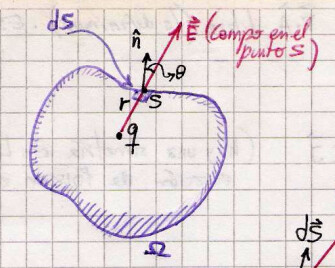
\includegraphics[width=0.35\textwidth]{images/fig_ft1_gauss.jpg}	 
	\end{center}
	\caption{}
	\label{fig_ft1_gauss}
\end{figure} 

El campo en el punto verifica
\[
	\vb{E} \cdot \hat{n} = q \frac{\cos(\theta)}{r^2}
\]
y teniendo en cuenta el diferencial de superifice $dS$
\[
	\vb{E} \cdot \hat{n} dS = q \frac{\cos(\theta)}{r^2} dS
\]
donde el factor $ \cos\theta dS / r^2 $ es el ángulo sólido subtendido por $dS$ desde el punto donde se halla $q$

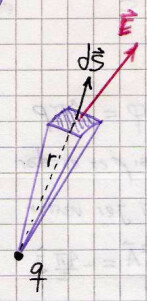
\includegraphics[width=0.15\textwidth]{images/fig_ft1_gauss_solid_angle.jpg}

Podemos escribir 
\[
	\vb{E} \cdot \hat{n} dS = q d\Omega
\]
donde $ d\Omega $ es el diferencial de ángulo sólido. Integrando para todo el volumen
\[
	\int_{S\equiv\partial V} \vb{E} \cdot \hat{n} \; dS = q \int_S d\Omega =
	\begin{cases}
	 0 \quad \textrm{carga exterior}\\
	 4\pi \quad \textrm{carga interior}
	\end{cases}
\]
y la integral es nula si la carga es exterior a $S$ o $4\pi$ si es interior.
En el caso de una cantidad de cargas internas se tendrá, evidentemente,
\[
	\int_S \vb{E} \cdot \hat{n} \; dS = 4\pi \sum_i q_i.
\]

Este hecho se conoce como La ley de Gauss y se expresa 
\[
	\int_S \vb{E} \cdot \hat{n} \; dS = 4\pi Q_n,
\]
donde $Q_n$ es la carga neta dentro de la superficie $S$. Al continuo pasa como 
\[
	\int_S \vb{E} \cdot \hat{n} \; dS = 4\pi \int_V \rho \: dV,
\]
de manera que usando el teorema de la divergencia se obtiene 
\[
	\int_V \divem{E} \; dV = \int_V 4\pi \rho \: dV,
\]
o bien
\[
	\divem{E} = 4\pi \rho.
\]

Lo que es vital en todo este razonamiento es el hecho de que el campo decaiga como $1/r^2$.
Luego, alguna `ley de Gauss' podrá aplicarse a cualquier campo con ese tipo de decaimiento.

Por otro lado si \vb{E} es el gradiente de un potencial $\phi$ la divergencia del campo
\[
	\divem{E} = \Nabla\cdot{(-\Nabla\phi)} = - \lapm\phi = 4\pi \rho
\]
conduce a la ecuación de Poisson para el potencial electrostático,
\[
	\lapm\phi = -4\pi \rho,
\]
cuyo caso particular en el caso $\rho=0$
\[
	\lapm\phi = 0,
\]
constituye la ecuación de Laplace.

Matemáticamente esto significa que la solución de la ecuación no homogénea (Poisson) es suma de 
una solución del homogéneo (Laplace) más una solución particular. 
La carga en el volumen está relacionada con la solución particular.

Por supuesto para resolver cualquiera de estas ecuaciones hace falta dar las correspondientes
condiciones de contorno. Usualmente serán de dos tipos: Dirichlet (valor del potencial en la
superifice) o Newmann (valor de la derivada normal del potencial sobre la superficie).

\subsection{Gauges}

Dado que $\divem{B}=0$ entonces existe un \vb{A} tal que 
\[
	\rotorm{A} = \vb{B}
\]
pero para caracterizar totalmente el \vb{A} tengo la libertad de definir a conveniencia
\[
	\divem{A} \equiv \; \textrm{``el gauge''}.
\]
Casos particulares importantes son el gauge de Coulomb,
\[
	\divem{A} = 0
\]
de manera que como 
\[
	\Nabla \times (\rotorm{A}) = \Nabla(\divem{A}) - \lapm{\vb{A}} = \frac{4\pi}{c}\vb{J}
\]
se llega para el potencial electromagnético, bajo el gauge de Coulomb, a que 
\[
	\lapm{\vb{A}} = - \frac{4\pi}{c}\vb{J} 
\]

	\begin{table}[ht]
	\centering
        \begin{tabular}{|c|c|}
		\hline
		Electrostática & Magnetostática \\
		\hline 
		 & \\
		$\displaystyle \vb{F}_{12} = \frac{q_1 q_2 ( \vb{x}_1 - \vb{x}_2 )}{ |\vb{x}_1 - \vb{x}_2|^3 } $
		& 
		$ \displaystyle d\vb{F}_{12} = \frac{1}{c^2} \frac{ I_1 d\vb{\ell}_1 \times J_2 d\vb{\ell}_2 \times ( \vb{x}_2 - \vb{x}_1 )}
		{ |\vb{x}_2 - \vb{x}_1|^3 }$
		\\
		 & \\
		\hline
		& \\
		$\displaystyle{\vb{E} = \int_{V'} \frac{\rho(\vb{x}')(\vb{x}-\vb{x}')}{|\vb{x}-\vb{x}'|^3} dV' 
		}$ & $\displaystyle{\vb{B} = \frac{1}{c} \int_{V'} \frac{\vb{J}(\vb{x}') \times 
		(\vb{x}-\vb{x}')}{|\vb{x}-\vb{x}'|^3} dV'}$ \\
		& \\
		\hline
		Ley de Gauss & Ley de Ampere \\
		& \\
		$\displaystyle{\int_S \vb{E}\cdot d\vb{S} = 4\pi Q_n}$ &
		$\displaystyle{\int_\Gamma \vb{B}\cdot d\vb{\ell} = \frac{4\pi}{c} I_c}$ \\
		& \\
		\hline
		Ecuaciones electrostáticas & Ecuaciones magnetostáticas \\
		&\\
		$\divem{E} = 4\pi\rho$ & $\divem{B} = 0$ \\
		&\\
		$\rotorm{E} = 0$ & $\rotorm{B} = \frac{4\pi}{c}\vb{J}$ \\
		& \\
		\hline
		& \\
		$\vb{E} = - \Nabla\phi$ & $\vb{B} = \rotorm{A}$ \\
		& \\
		\hline
		\end{tabular} 
		\caption{Recetario de ecuaciones básicas para la electrostática y la
		magnetostática.}
	\end{table} 

\notamargen{Estos comentarios sobre vectores irán en el apéndice matemático vectorial.}
La operación de tomar rotor y el producto vectorial cambian el carácter de los vectores: de
polares pasan a axiales y viceversa.

El laplaciano es la divergencia del gradiente, dos operaciones que no cambian el carácter de
un vector. Luego, el laplaciano preserva la simetría.

La fuerza general sobre una distribución de carga es
\[
	\vb{F} = \int_{V'} \rho \vb{E} \: dV' + \frac{1}{c} \int_{V'} \vb{J} \times \vb{B} \: dV'. 
\]

\notamargen{
A partir de la tabla hay mucho para mencionar. Por ejemplo, el hecho de la separación total
de fenómenos, que la fuerza magnética es una diferencial (no hay cargas puntuales magnéticas),
que el potencial en un caso es escalar mientras que en el otro es vectorial, etc.
}

\subsection{Delta de Dirac}

Una densidad de carga puntual se puede escribir mediante una delta de Dirac de acuerdo a
\[
	\rho(\vb{x}') = q\: \delta (\vb{x} - \vb{x}') = \begin{cases}
	                                               0 \qquad \vb{x} \neq \vb{x}' \\
	                                               \infty \qquad \vb{x} = \vb{x}'\\
	                                              \end{cases}
\]
siendo las dimensiones de la delta las de $1/L^3$ y cumpliéndose 
\[
	\int_{V'} \delta (\vb{x} - \vb{x}') dV' = 1.
\]

La delta de Dirac se puede aproximar con ciertas funciones matemáticas con gráficas como el 
siguiente 

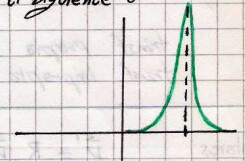
\includegraphics[width=0.25\textwidth]{images/fig_ft1_delta_dirac.jpg}

La delta de Dirac cumple las siguientes propiedades
\[
	\int f(\vb{x}) \delta(\vb{x} - \vb{x}_0) dx = f(\vb{x}_0)
\]
\[
	\int f(\vb{x}) \delta' (\vb{x} - \vb{x}_0) dx = -f'(\vb{x}_0)
\]
\[
	\int f(\vb{x}) \delta^n (\vb{x} - \vb{x}_0) dx = (-1)^n f^n(\vb{x}_0)
\]
\[
	\delta[f(x)] = \frac{\delta(\vb{x}-\vb{x}_0)}{|f'(\vb{x}_0)|} \qquad \qquad f(\vb{x}_0) = 0
\]

En coordenadas cartesianas es
\[
	\delta(\vb{x}-\vb{x}_0) = \delta(x-x_0)(y-u_0)(z-z_0)
\]
y para curvilíneas, como el elemento diferencial y el de volumen son  
\[
	d\vb{x} = h_1 dq_1 \hat{e}_1 + h_2 dq_2 \hat{e}_2 + h_3 dq_3 \hat{e}_3 
	\qquad 	dV = h_1 h_2 h_3 dq_1 dq_2 dq_3
\]
se tiene
\[
	\delta (\vb{x} - \vb{x}') = \frac{1}{h_1h_2h_3} \delta(q_1-q_1') \delta(q_2-q_2') \delta(q_3-q_3')
\]
donde $q_1, q_2$ y $q_3$ son coordenadas curvilíneas generales y $h_1h_2h_3$ es el jacobiano
de la transformación.
Puntualmente para coordenadas esféricas se tiene 
\[
	\delta (\vb{x} - \vb{x}') = \frac{1}{r^2 \sin\theta} 
	\delta(r-r') \delta(\theta-\theta') \delta(\varphi-\varphi')
\]
donde no está definido para $\theta=0$. Si $r_0=0$ entonces se tiene 
\[
	\delta(\vb{x}) = \frac{\delta(r)}{4\pi r^2}
\]
que involucra un factor de normalización.

Para un casquete esférico se tendrá $\rho(\vb{x}) = \sigma \delta(r-R) $ y para una corriente
circulando por un plano como ilustra la figura

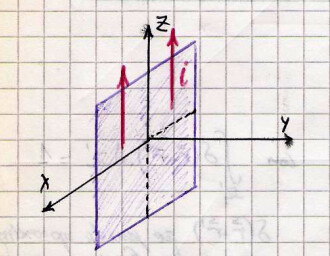
\includegraphics[width=0.25\textwidth]{images/fig_ft1_deltas_ejemplos.jpg}
se tiene $\vb{J} = g \delta(y) \hat{z}$. Estas deltas, al ser unidimensionales tienen unidades
de $1/L^{-1}$ de manera que las otras unidades serán llevadas por $\sigma$ y $g$.

\subsection{Vectores polares y axiales ante transformaciones}

Las transformaciones propias son aquellas con determinante 1 y las impropias las que tienen determinante
distinto de 1.
Entonces, para un vector polar $\vb{p}$ y siendo $R$ la matriz de la transformación y $|R|$ su determinante, 
se tiene 
\[
	\vb{p}' = R \: \vb{p},
\]
mientras que para un vector axial \vb{a}
\[
	\vb{a}' = |R| R \: \vb{a}.
\]

Aquí se ve que ante una transformación propia ambos vectores transforman igual pero ante una impropia 
hay un cambio asociado al determinante.

Un vector polar sufre reflexión especular mientras que un vector axial ({\it pseudovector})
sufre una antireflexión especular. Ver la figura.

\begin{figure}[htb]
	\begin{center}
	\includegraphics[width=0.6\textwidth]{images/fig_ft1_reflexvect.pdf}	 
	\end{center}
	\caption{A la izquierda está el comportamiento polar mientras que a la derecha
	se halla el comportamiento axial.}
\end{figure} 

Para un campo escalar, como podría ser la temperatura $T(\vb{x})$ una rotación deja invariante el valor
del campo 

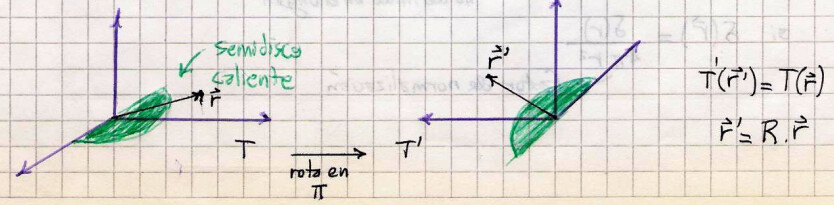
\includegraphics[width=0.8\textwidth]{images/fig_ft1_rotacion_escalar.jpg}

En el caso de un campo vectorial 

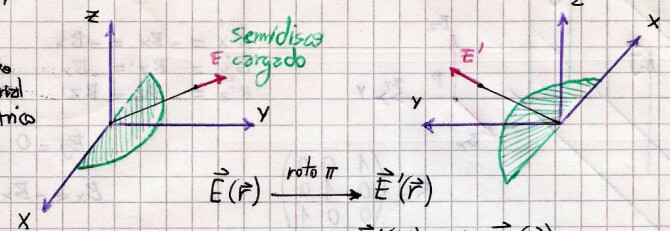
\includegraphics[width=0.8\textwidth]{images/fig_ft1_rotacion_vectorial.jpg}\\
se ve que 
\[
	\vb{E}'(\vb{x}') = R\vb{E}( R\vb{x}).
\]

En el caso de una simetría por reflexión como la de la figura 

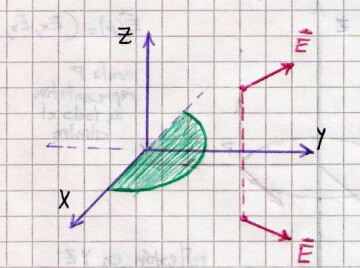
\includegraphics[width=0.4\textwidth]{images/fig_ft1_reflexion_vectorial.jpg}\\
el campo en una situación simétrica cumplirá 
\[
	\vb{V}(\vb{x}') = R \vb{V}(\vb{x})
\]
mientras que un campo escalar sería $T(\vb{x}')=T(\vb{x})$.

% Ejemplo eléctrico

\begin{ejemplo}{\bf Ejemplo de problema simétrico (eléctrico)}

Consideremos un plano infinito cargado con una densidad de carga $\sigma$, según se
ve en la figura bajo estas líneas. 
La idea es que el campo en un punto $P$ será 
\[
	\vb{E}(P) = (E_x, E_y, E_z), 
\]
es decir que en principio tendrá los tres componentes.

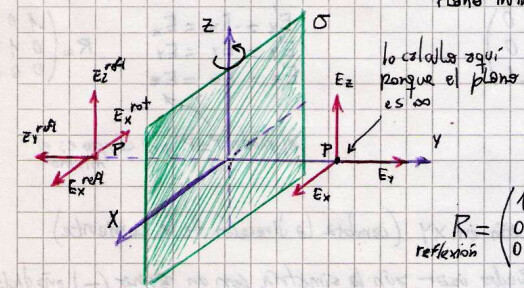
\includegraphics[width=0.4\textwidth]{images/fig_ft1_ej_plano_cargado.jpg}

Del otro lado del plano la situación es la misma de manera que se tiene una simetría de 
reflexión en $xz$. La matriz de una reflexión es 
\[
	R = \begin{pmatrix}
		1 & 0 & 0 \\
		0 & -1 & 0 \\
		0 & 0 & 1
	\end{pmatrix}
\]
y entonces se tienen las relaciones (compruébese en la figura)
\be
	E_x' = E_x, \qquad E_y' = -E_y, \qquad E_z' = E_z.
	\label{simetria_refl}
\ee

Luego, otra simetría es sencillamente rotar el plano un ángulo $\pi$ en torno a $\hat{z}$,
y esta rotación será \notamargen{poner matriz de rotación en apéndice}
\[
	R = \begin{pmatrix}
		-1 & 0 & 0 \\
		0 & -1 & 0 \\
		0 & 0 & 1
	\end{pmatrix}
\]
que implica 
\be
	E_x' = -E_x, \qquad E_y' = -E_y, \qquad E_z' = E_z.
	\label{simetria_rot}
\ee

Como ambas simetrías conllevan a la misma situación física, deben ser ciertas las relaciones 
\eqref{simetria_refl} y \eqref{simetria_rot} de modo que como $E_x = - E_x$ se debe cumplir 
que $E_x = 0$.

Se puede hacer el mismo razonamiento para la simetría de reflexión en torno a $xy$ puesto que
dicho plano separa dos semiespacios especularmente idénticos. En este caso como $P$ se halla
sobre dicho plano basta una rotación en un ángulo de $2\pi$, que deja el campo en el mismo
sitio para obtener la relación $E_z = - E_z$ lo cual implica que $\vb{E} = E_y \hat{y}$.
\end{ejemplo}

% Ejemplo magnético 

\begin{ejemplo}{\bf Ejemplo de problema simétrico (magnético)}

Consideremos un plano infinito por el cual circula una corriente cuya densidad de corriente \vb{J}
está mostrada en la figura bajo estas líneas. 
La idea es que el campo magnético \vb{B} en un punto $P$ será 
\[
	\vb{B}(P) = (B_x, B_y, B_z), 
\]
es decir que en principio tendrá los tres componentes.
 
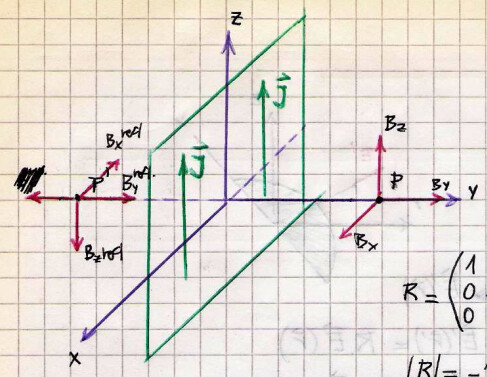
\includegraphics[width=0.4\textwidth]{images/fig_ft1_ej_plano_corriente.jpg}

Dado que este campo es un pseudovector, debe reflejarse {\it mal} en el plano, como se ilustra en
la figura. La reflexión en el plano $xz$ lleva a 
\be
	B_x' = -B_x, \qquad B_y' = B_y, \qquad B_z' = -B_z,
	\label{Bsimetria_refl}
\ee
que proviene de la matriz de reflexión $R$ del caso anterior (es la misma porque giramos en el
mismo sentido el mismo plano) a la cual se le ha multiplicado el determinante $|R|=-1$ de la misma
puesto que el campo \vb{B} es un pseudovector.

La rotación en torno a un ángulo $\pi$ del plano es también una simetría, representada por la misma
matriz de rotación $R$ del ejemplo anterior por lo cual se tendrán 
\be
	B_x' = -B_x, \qquad B_y' = -B_y, \qquad B_z' = B_z,
	\label{Bsimetria_rot}
\ee 
de lo cual se deduce que $ B_y = B_z = 0 $. El campo magnético sólo puede tener componente en $\hat{x}$,
es decir que se escribirá como $\vb{B} = B_x \hat{x}$.
Este hecho también puede deducirse cualitativamente utilizando la regla de la mano derecha.
\end{ejemplo}


\begin{ejemplo}{\bf Hilo cargado e hilo con corriente}

Consideraremos ahora dos situaciones geométricas idénticas (un hilo infinito) pero en primer lugar el
caso en que está cargado uniformemente y en segundo lugar el caso en que por el mismo circula una
corriente estacionaria $i$. 

En el caso del hilo cargado se quiere determinar las simetrías del campo $\vb{E}$ en un punto $\vb{P}$,

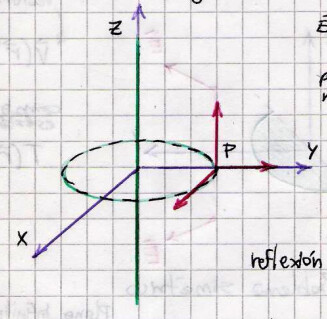
\includegraphics[width=0.4\textwidth]{images/fig_ft1_ej_hiloE.jpg}

El punto \vb{P} es representativo de todo el cilindro. La simetría de reflexión en $xy$ no hace que el
punto cambie ($\vb{P}' = \vb{P}$) pero el campo debe reflejarse, de lo cual se tiene 
\[
	E_x' = E_x, \qquad E_y' = E_y, \qquad E_z' = -E_z.
\]
Luego, la rotación en ángulo $2\pi$ implica que $E_z = -E_z$ y por ende el componente $z$ debe ser nulo.

Por otra parte, la simetría de reflexión en $yz$ de igual manera lleva a $E_x = -E_x$ de forma que
el campo \vb{E} de un hilo cargado solo tendrá componentes en $\hat{y}$.

En el caso del hilo con una corriente que circula por el mismo se debe notar que ahora la corriente tiene
dirección con lo cual la simetría de reflexión en $xy$ se verifica si incorporamos un signo menos que dé
cuenta del cambio en la dirección de la corriente

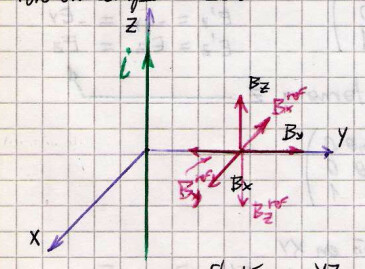
\includegraphics[width=0.4\textwidth]{images/fig_ft1_ej_hiloB.jpg}

Entonces por una parte tenemos la reflexión que, luego del añadido del signo extra, da las igualdades 
\[
	B_x' = B_x, \qquad B_y' = B_y, \qquad B_z' = -B_z,
\]
que al combinarse con las que resultan de que los puntos son el mismo $\vb{P}=\vb{P}'$ (o digamos que 
giramos en ángulo $2\pi$) resultan en que $B_z = -B_z$ y por ende $B_z$ es nulo.

La reflexión en $yz$ no requiere el signo menos extra por el cambio de la corriente, así que da sencillamente 
\[
	B_x' = B_x, \qquad B_y' = -B_y, \qquad B_z' = -B_z,
\]
y luego la igualdad de puntos establece 
\[
	B_x' = B_x, \qquad B_y' = B_y, \qquad B_z' = B_z,
\]
de modo que, igualando ambas expresiones, tiene que ser $ B_y = B_z = 0 $. Entonces el campo $\vb{B}$ sólo
tiene componentes en $\hat{x}$, es un campo anular.
\end{ejemplo}

\notamargen{En estos ejemplos creo que es más beneficiosa la notación de la carpeta, ecuaciones `triples'.}


Como se vió en el ejemplo anterior, una reflexión más una rotación permite eliminar componentes 
de campo.


Una simetría más una rotación-traslación permite eliminar dependencias.

Lo primero que debe hacerse es escribir bien la \vb{J} a partir del dato de la corriente
(que es el que se suele tener) mediante
\[
	i = \int_S \vb{J} \cdot d \vb{S}
\]
En cambio, para \vb{A} es más fácil usar
\[
	\vb{B} = \rotorm{A}
\]
y despejar de aquí la ecuación diferencial que emplear
\[
	\vb{A} = \frac{1}{c} \int_V \frac{\vb{J}}{|\vb{x}-\vb{x}'|} dV
\]


\section{El potencial vector}

Por la ley de Biot y Savart, el campo \vb{B} debido a una densidad 
de corriente en un volumen puede obtenerse a partir de
\be
	\vb{B} = 
	\frac{1}{c} \int_{V'} \frac{\vb{J}(\vb{x}') \times (\vb{x}-\vb{x}')}{|\vb{x}-\vb{x}'|^3} dV' .
	\label{campo_B}
\ee

Utilizando la identidad de \eqref{ident_vec_posicion}, con el gradiente respecto del punto campo,
y la identidad vectorial
\[
	\Nabla \times (\phi \vb{F} ) = \phi \rotorm{F} - \vb{F} \times \Nabla \phi
\]
la expresión \eqref{campo_B} para el campo magnético resulta en 
\[
	\vb{B} = \Nabla_x \times \frac{1}{c} \int_{V'} \frac{\vb{J}(\vb{x}')}{|\vb{x}-\vb{x}'|} dV'
\]
de modo que
\be
	\vb{A} = \frac{1}{c} \int_{V'} \frac{\vb{J}(\vb{x}')}{|\vb{x}-\vb{x}'|} dV'
	\label{potvec}
\ee
pero como el potencial vector se define a menos del gradiente de un escalar, resulta
\[
	\vb{A}' \equiv \vb{A} + \Nabla \psi
\]
es tan buen potencial vector como \vb{A} puesto que los rotores verifican $\rotorm{A}=\rotorm{A}'=\vb{B}$,
de lo cual extraemos en conclusión que el potencial vector está definido a menos del gradiente de una
función escalar.
\notamargen{Reacomodar estas cosas.}

Cada componente de \vb{A} en el caso de que $\Nabla\psi=0$ puede verse como una integral de Poisson.

Ahora bien, si se toma el rotor del campo \vb{B}, lo cual es tomar el rotor de \vb{A}, se tiene
\[
	\rotorm{B} = \Nabla\times\left( \frac{1}{c} \int_{V'} \frac{\vb{J}(\vb{x}')}{|\vb{x}-\vb{x}'|} dV' \right)
\]
y usando la identidad del rotor de un rotor (ver apéndices XXX) resulta descompuesto en dos términos de
acuerdo a
\[
	\rotorm{B} = 
	\Nabla\left( \Nabla \cdot \left[ \frac{1}{c} 
		\int_{V'} \frac{\vb{J}(\vb{x}')}{|\vb{x}-\vb{x}'|} dV' \right] \right) -
	\nabla^2 \left( \frac{1}{c} \int_{V'} \frac{\vb{J}(\vb{x}')}{|\vb{x}-\vb{x}'|} dV' \right),
\]
el gradiente de una divergencia y el laplaciano de un vector. Trabajaremos cada uno de ellos por 
separado. 

Dado que la divergencia es con respecto a las coordenadas de \vb{x} y la integración es con respecto
a las coordenadas \vb{x}' puede introducirse la misma bajo el signo integral y entonces
\[
	I_1 = \frac{1}{c} 
		\int_{V'} \vb{J}(\vb{x}') \Nabla \cdot \left[ \frac{ 1 }{|\vb{x}-\vb{x}'|} \right] dV'
		= - \frac{1}{c} 
		\int_{V'} \vb{J}(\vb{x}') \Nabla' \cdot \left[ \frac{ 1 }{|\vb{x}-\vb{x}'|} \right] dV'
\]
donde la última igualdad se debe al cambio de las coordenadas contra las cuales se deriva.
Ahora notando la siguiente expresión para la divergencia del integrando en el potencial vector,
\[
	\Nabla' \cdot \left[ \frac{ \vb{J}(\vb{x}') }{|\vb{x}-\vb{x}'|} \right] =
	\frac{ \Nabla' \cdot \vb{J}(\vb{x}') }{|\vb{x}-\vb{x}'|} +
	 \vb{J}(\vb{x}') \cdot \Nabla' \left[ \frac{ 1 }{|\vb{x}-\vb{x}'|} \right]
\]

Considerando que $\Nabla'\cdot\vb{J}(\vb{x}')=0$, lo cual se verifica si
la corriente es estacionaria se tiene 
\[
	I_1 = - \frac{1}{c} 
	\int_{V'} \Nabla' \cdot \left[ \frac{ \vb{J}(\vb{x}')  }{|\vb{x}-\vb{x}'|} \right] dV'
\]
expresión a la cual se puede aplicar el teorema de la divergencia en una superficie 
$ S' = \partial V' $ que englobe completamente a la distribución de corrientes dada por 
$\vb{J}$ (y esto siempre se puede hacer si \vb{J} está acotada) resultando en 
\[
	I_1 = \frac{1}{c} \int_{S'} 
	\frac{ \vb{J}(\vb{x}')  }{|\vb{x}-\vb{x}'|} \cdot \hat{n} dS' = 0.
\]

El segundo término es 
\[
	I_2 = \nabla^2 \left( \frac{1}{c} \int_{V'} \frac{\vb{J}(\vb{x}')}{|\vb{x}-\vb{x}'|} dV' \right)
\]
donde el laplaciano, por la misma razón, también puede ser llevado dentro de la integral lo 
cual resulta en 
\[
	I_2 = \frac{1}{c} \int_{V'} \vb{J}(\vb{x}') \: \nabla^2 \left( \frac{1}{|\vb{x}-\vb{x}'|} \right) dV'
	= \frac{4 \pi }{c} \int_{V'} \vb{J}(\vb{x}') \: \delta( \vb{x}-\vb{x}') dV',
\]
luego de utilizar el valor del laplaciano de la diferencia entre puntos campo y fuente. La
integral es nula salvo en el caso en el cual el punto \vb{x} se halle dentro de $V'$, lo cual 
suponemos que es cierto obteniéndose entonces 
\[
	I_2 = - \frac {4 \pi} {c} \vb{J}(\vb{x}).
\]

Juntando todos los resultados de estas excursiones, arribamos a 
\[
	\rotorm{B} = \frac{4 \pi} {c} \vb{J}(\vb{x}).
\]

Integrando esta ecuación de Maxwell sobre una superficie $S$ cuya frontera es una curva
cerrada $\Gamma$ se tiene 
\[
	\int_S \rotorm{B} \cdot d\vb{S} = \frac{4\pi}{c} \int_S \vb{J}(\vb{x}) \cdot d\vb{S}
\]
y por el teorema de Stokes arribamos a
\[
	\int_{\Gamma\equiv\partial S} \vb{B}\cdot d\vb{\ell} = \frac{4\pi}{c} I_\Gamma
\]
que es la ley de Ampere. Notemos que $I_\Gamma$ es la corriente concatenada por el lazo $\Gamma$.

Además, volviendo a la identidad vectorial del doble rotor, 
\[
	\rotorm{B} = \Nabla\times(\rotorm{A}) = \Nabla(\divem{A}) - \nabla^2 \vb{A} = \frac{4\pi}{c}\vb{J}
\]
que se simplifica utilizando el gauge de Coulomb, $\divem{A}=0$, para llegar a 
\[
	\nabla^2 \vb{A} = -\frac{4\pi}{c}\vb{J},
\]
que es una ecuación de Poisson vectorial para la magnetostática.

Magnetostática y electrostáctica son gobernadas por ecuaciones de Poisson para potenciales $\vb{A},\phi$ y
el problema entonces se reduce a resolverlas para luego hallar los campos por derivación.

\begin{ejemplo}{\bf Ejemplo de Gauss law y Ampere law}

Se tiene un hilo cargado con una densidad lineal de carga $ \lambda $, tomando una superficie gaussiana
cilindrica coaxial y concéntrica con el mismo 

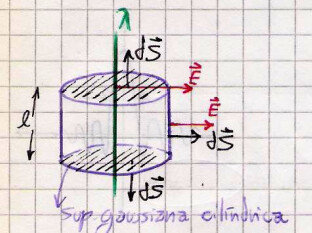
\includegraphics[width=0.4\textwidth]{images/fig_ft1_gausslaw.jpg}

se tiene 
\[
	\int \vb{E}\cdot d\vb{S} = 4 \pi Q,
\]
y dada la forma del campo en cada superficie se tiene
\[
	E 2 \pi r \ell = 4 \pi \lambda \ell
\]
de modo que 
\[
	E = \frac{2 \lambda}{r}.
\]

En el caso de un toro por el cual circula una corriente $i$ en cada vuelta de la espira se definen dos
circuitos $\Gamma_1$ y $\Gamma_2$ según al figura debajo

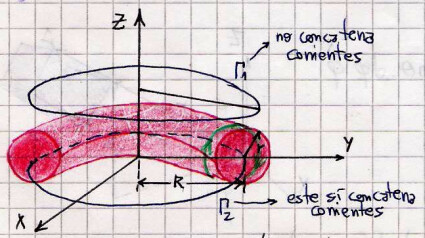
\includegraphics[width=0.4\textwidth]{images/fig_ft1_amperelaw.jpg}

El campo $\vb{B}$ estará en $\phiver$ y además no depende de $\vp$ por la simetría (en coordenadas
cilíndricas), entonces para un dado $r_0$ y $z_0$ será una constante en $\phiver$.
Entonces
\[
	\int_\Gamma \vb{B}\cdot d\vb{\ell} = \frac{4 \pi }{c} I_c
\]
y para los circuitos de la figura 
\[
	\int_{\Gamma_1} \vb{B}\cdot d\vb{\ell} = 0 \qquad \vb{B} = 0
\]
de modo que el campo magnético será nulo fuera. En cambio, dentro
\[
	\int_{\Gamma_1} \vb{B}\cdot d\vb{\ell} = \frac{4\pi}{c}Ni \qquad B = \frac{2Ni}{Rc}
\]

\notamargen{Estaría bueno hacer un análisis fino de las aproximaciones, hacer el cálculo
posta de los campos magnéticos y ver que las consideraciones de simetría funcionan.
Este ejemplo, pese a lo boludo, es muy ilustrativo.}

\end{ejemplo}


\section{Resolviendo problemas de potencial}

Estaremos interesados en resolver las ecuaciones de Poisson y de Laplace en un cierto recinto.
Para tener soluciones únicas necesitaremos condiciones de contorno de tipo Dirichlet o de tipo Newmann (derivada
normal en el contorno).


\subsection{Unicidad de problemas de potencial}

La unicidad de la solución permite la fabricación de problemas equivalentes para otras soluciones.
Si dos problemas satisfacen iguales condiciones de contorno entonces en el recinto encerrado por
ese contorno tienen igual solución.

Si en un recinto $R$
\be
	\phi_1|_{cont} = \phi_2|_{cont}
	\label{potnounico}
\ee
pero se da para el interior de $R$ que $\phi_1\neq\phi_2$ entonces se tiene sucesivamente
\[
	U \equiv \phi_1 - \phi_2 \qquad \qquad \Nabla U = \Nabla \phi_1 - \Nabla \phi_2
\]
\[
	\lapm{U} = \lapm{\phi_1} - \lapm{\phi_2} = -4\pi \rho + 4\pi\rho = 0
\]
\[
	\Nabla\cdot\left( U\Nabla U \right) = U\left( \Nabla\cdot\Nabla U \right) + \Nabla U \cdot \Nabla U
\]
\[
	\int_V \Nabla\cdot\left( U\Nabla U \right) dV = 
	\int_V U \lapm{U}  + (\lapm{U})^2 dV =  \int_V (\lapm{U})^2 dV
\]
llegando al último miembro porque el potencial $U$ cumple la ecuación de Laplace. Luego,
\[
	\int_V (\lapm{U})^2 dV = \int_S U\Nabla{U} \cdot d\vb{S} = 0
\]
habiéndose pasado a la integral de superficie por el teorema de la divergencia y anulando 
el valor global porque 
$U$ en el contorno es nula (recuérdese \eqref{potnounico}). Además, 
\[
	\Nabla{U} \cdot d\vb{S}  \longrightarrow \left.\dpar{U}{\hat{n}}\right|_{cont}
\]
luego,
\[
	\Nabla U = 0 \qquad \Nabla\phi_1 = \Nabla\phi_2 
\]
y entonces
\[
	\phi_1 = \phi_2 .
\]
a menos, por supuesto, de una constante.

\notamargen{Veo la idea acá pero esto hay que hacerlo con mucho cuidado.
Tal vez garabatear en papel y pasar los pasos importantes aquí.
Utilizar claramente las condiciones de contorno; Dirichlet o Newmann.}


Los problemas que siguen parecen ser correspondientes a cálculo de campos a lo F3, de manera que
tendrán que reubicarse luego. Suponemos que son guía 1.
\begin{ejemplo}{\bf Problema 6}

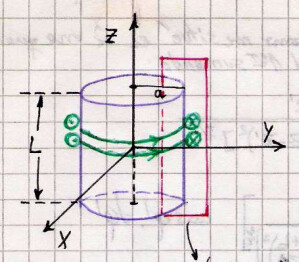
\includegraphics[width=0.3\textwidth]{images/fig_ft1_setproblemasG1_1.jpg}

La integral del campo magnético es
\[
	\vb{B}(\vb{x}) = \frac{1}{c}\int_\Omega  
	\frac{ \vb{J}(\vb{x}) \times (\vb{x}-\vb{x}')}{|\vb{x}-\vb{x}'|^3} d\Omega
\]
pero primeramente se busca obtener la corriente, cuya distribución es proporcional a la delta
de Dirac con alguna constante de proporcionalidad que hay que hallar. Entonces
\[
	I_T = \int_S \vb{J}\cdot d\vb{S} = \int_0^\infty \int_{-L/2}^{L/2} \alpha \delta(y-a) dy dz =
	\alpha \int_{-L/2}^{L/2} dz = \alpha L = I n L
\]
de lo cual se obtiene $\alpha = n L$ y donde se ha usado $n=N/L$.

Luego,
\[
	\vb{B}(\vb{x}) = \frac{1}{c} \int_{-L/2}^{L/2} \int_0^{2\pi} \int_0^a 
	\frac{ n I \delta(r'-a) r' \phiver \times ( -r'\cos\vp'\xver - r'\sin\vp'\yver + (z-z')\zver) }
	{({r'}^2 + [z-z']^2)^{3/2}} \: dr' d\vp' dz'
\]
y colapsando la delta en $r$,
\[
	\vb{B}(\vb{x}) = \frac{n I}{c} \int_{-L/2}^{L/2} \int_0^{2\pi} 
	\frac{ a' \phiver \times ( -a'\cos\vp'\xver - a'\sin\vp'\yver + (z-z')\zver) }
	{({a'}^2 + [z-z']^2)^{3/2}} \: d\vp' dz'
\]
donde el producto vectorial requiere previamente convertir $\phiver$ a cartesianas.
Entonces, usando la regla mnemotécnica sabida,
\[
	\begin{vmatrix}
	\xver & \yver & \zver \\
	 -\sin\vp' & -\cos\vp' & 0 \\
	 -a\cos\vp' & -a\sin\vp' & (z-z')\\
	\end{vmatrix}
	= \cos\vp'(z-z')\xver + \sin\vp'(z-z')\yver + a\zver
\]

Las integrales en $\cos\vp'$ y $\sin\vp'$ dan cero porque son trigonométricas entre 0 y 2$\pi$.
Luego
\[
	\vb{B}(0,0,z) = \frac{n I 2 \pi a^2}{ c } \int_{-L2}^{L/2} \frac{ dz'}{( a^2 + [z-z']^2)^{3/2}} \: \zver =
	\frac{2 \pi n I}{c } \left( \frac{L/2 + z}{a^2 + (z+L/2)^2 } + \frac{L/2 - z}{a^2 + (L/2 - z)^2} \right)
\]
\notamargen{Acá parece que se simplificaba el $a^2$.}
y se obtiene 
\[
	\vb{B}(0,0,z) = \frac{2 \pi n I}{c}\left( \cos\theta_2 + \cos\theta_1 \right)
\]

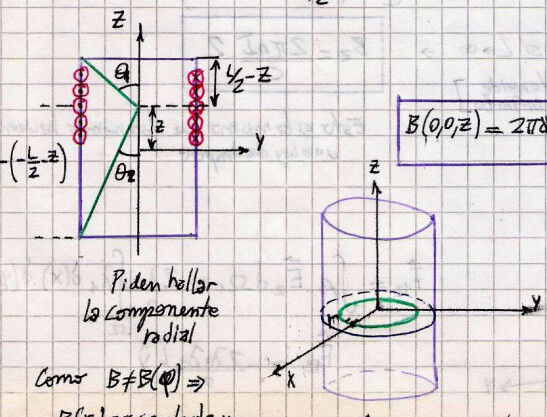
\includegraphics[width=0.4\textwidth]{images/fig_ft1_setproblemasG1_2.jpg}

Piden hallar la componente radial. Como $B$ no depende de $\vp, B(r_0)$ es constante y entonces situándose
en $\xver$ sabré que es válido en un círculo $r$
\[
	\vb{B}(\vb{x}) =  \frac{nIa}{c}\int_{-L2}^{L/2} \int_0^{2\pi} 
	\frac{\hat{\vp}\times (\vb{x}-\vb{x}')}{|\vb{x}-\vb{x}'|^3} d\vp'dz
\]
Ahora es
\[
	\vb{x}-\vb{x}' =
\]
pero como requiero únicamente el campo en $\rver$ me interesará la parte en $\zver$ pués $\phiver\times\zver=\rver$.
\[
	\rver = \cos\vp'\xver + \sin\vp'\yver,
\]
pero como estoy situado en $\xver$ me quedo únicamente con el primer sumando.
\[
	B_x(r,z) = \frac{anI}{c}\int_{-L2}^{L/2} \int_0^{2\pi} 
	\frac{ (z-z')\cos\vp' }{ ( a^2 + r^2 - 2ar\cos\vp + [z-z']^2 )^{3/2} } \: d\vp' dz' 
\]
y definiendo $b^2 \equiv a^2 + r^2 - 2ar\cos\vp$, se puede hacer la integral en $z'$ y  
\[
	B_x(r,z) = \frac{anI}{c} \int_0^{2\pi} 
	\left[ \frac{ 1 }{ b^2 + [z-L/2]^2 )^{1/2} } -  \frac{ 1 }{ b^2 + [z+L/2]^2 )^{1/2} }
	\right] \cos\vp' \: d\vp' dz' 
\]

Pero b es función de $\vp$ de modo que conviene aproximar con $L\gg a$ ( $r,a \ll L$, entonces $b \ll L$ y puedo
expandir con Taylor y $z \ll L$.
\[
	\frac{1}{\sqrt{ b^2 + (z \pm L/2 )^2 }} = \frac{2}{L} \frac{1}{\sqrt{ 1 + 4b^2/L^2 + 4z^2/L^2 \pm 4z/L }}
\]
y definiendo $\alpha \equiv 4b^2/L^2 + 4z^2/L^2$ y $\beta \equiv 4z/L$ se tiene 
\[
	\frac{2}{L}( \frac{1}{\sqrt{1 +(\alpha - \beta)}} - \frac{1}{\sqrt{\alpha + \beta}} ) \approx 
	1 - \frac{1}{2}(\alpha + \beta) + \frac{3}{8}(\alpha - \beta)^2 - 1 + \frac{1}{2}(\alpha + \beta) - \frac{3}{8}(\alpha + \beta)^2
	= \beta \left(1 - \frac{3}{2}\alpha \right)
\]
y regresando al cálculo de B
\[
	B_x(r,z) = \frac{a n I}{c} \int_0^{2\pi} \frac{2}{L}
	\left( \frac{4z}{L} \left( 1 - \frac{3}{2} \left[  \frac{4}{L^2}( r^2 - 2 a r \cos\vp'+ a^2 + z^2 ) 
	\right] \right) \right)
	\cos\vp'\:d\vp' 
\]
\[
	B_x(r,z) = \frac{8aznI}{L^2c}\frac{12 ar\pi}{L^2} = \frac{96 \pi n I}{c}\Frac{a^2zr}{L^4}
\]
\notamargen{Anoté que el término que multiplica al 3/2 sería un $\alpha$ (supongo ``el'' $\alpha$).
Chequearlo.}
y junto con
\[
	B_z = \frac{2 \pi n I}{ c }( \cos\theta_1 + \cos\theta_2 ).
\]

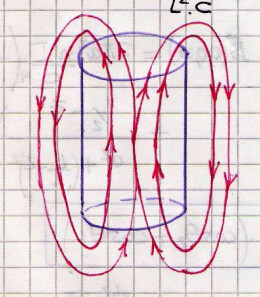
\includegraphics[width=0.2\textwidth]{images/fig_ft1_setproblemasG1_3.jpg}

Si $L \to \infty$ (caso de solenoide infinito) se tiene 
\[
	B_z = \frac{4 \pi n I}{ c },
\]
que es lo mismo que se obtiene haciendo una ley de Ampere.
 
\end{ejemplo}

\begin{ejemplo}{\bf Problema 8}

Acá esto es apenas un comentario.

\notamargen{Para un hilo cargado es $E = 2\lambda /r$}

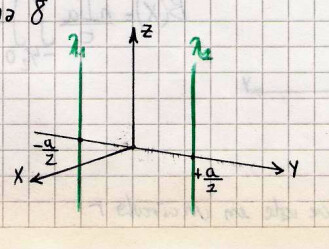
\includegraphics[width=0.3\textwidth]{images/fig_ft1_setproblemasG1_4.jpg} 

\[
	\vb{F}_{12} = \int \rho_1 \vb{E}_1 d\Omega_1 =
	\frac{2 \lambda_2 }{a} \int_\Omega \lambda_1 \delta(x) \delta(y+a/2) d\Omega_1
\]
\[
	\vb{F}_{12} = - \frac{2 \lambda_1 \lambda_2 }{a} L \yver
\]
 
\end{ejemplo}

\begin{ejemplo}{\bf Problema 5}

El potencial
\[
	\phi(r) = \frac{e}{r} \left( 1 + \frac{r}{a} \right) \euler^{-2r/a}
\] 
revienta en cero. No obstante se puede separar en dos potenciales uno de los cuales revienta y el otro no,
\[
	\phi(r) = \frac{e}{r} \euler^{-2r/a} +  \frac{e}{a} \euler^{-2r/a}
\]
donde el primer término es Yukawa, sumando y restando $e/r$ y agrupando
\[
	\phi(r) = \frac{e}{r} \left( \euler^{-2r/a} - 1\right) + \frac{e}{a} \euler^{-2r/a} + \frac{e}{r}
\]
donde el último término es el potencial de una carga en el origen que proviene de una densidad de
carga $\rho = e\delta(\vb{x})$. Definiendo al primer término como $\phi_1$ se puede despejar $\rho$
desde la ecuación de Poisson $ \lapm{\phi} = -4\pi \rho$,
\[
	\rho = -\frac{1}{4\pi r} \frac{1}{r} \dpar[2]{}{r}(r\phi_1)
\]
o bien
\[
	\rho = -\frac{1}{a^2 \pi r} \frac{e}{r} r \euler^{-2r/a}, 
\]
y hemos averiguado la densidad de carga de cada parte.

Entonces, por ser átomo neutro
\[
	Q = \int_V \rho dV + e = 0,
\]
y la integral puede hacerse en esféricas porque la dependencia es solamente en $r$.

\end{ejemplo}




% \bibliographystyle{CBFT-apa-good}	% (uses file "apa-good.bst")
% \bibliography{CBFT.Referencias} % La base de datos bibliográfica

\end{document}
